\section{Automatic Image Processing}

In this section we provide detailed hands-on instruction on automatic image processing within 2dx \cite{scherer20142dx_automator}, including on-the-fly image drift-correction. The here described pipeline is optimised for data recorded on a direct electron detector, such as the Gatan K2 summit. 

\subsection{Optimal image acquisition}

\subsection{Real-time motion-correction}

https://github.com/C-CINA/2dx/wiki/Automatic-Drift-Correction-C-CINA-setup

\subsection{Automation setup}

\subsection{2dx\_automator}

asdf  \autoref{fig:auto} adf.

\begin{figure}
	\centering
	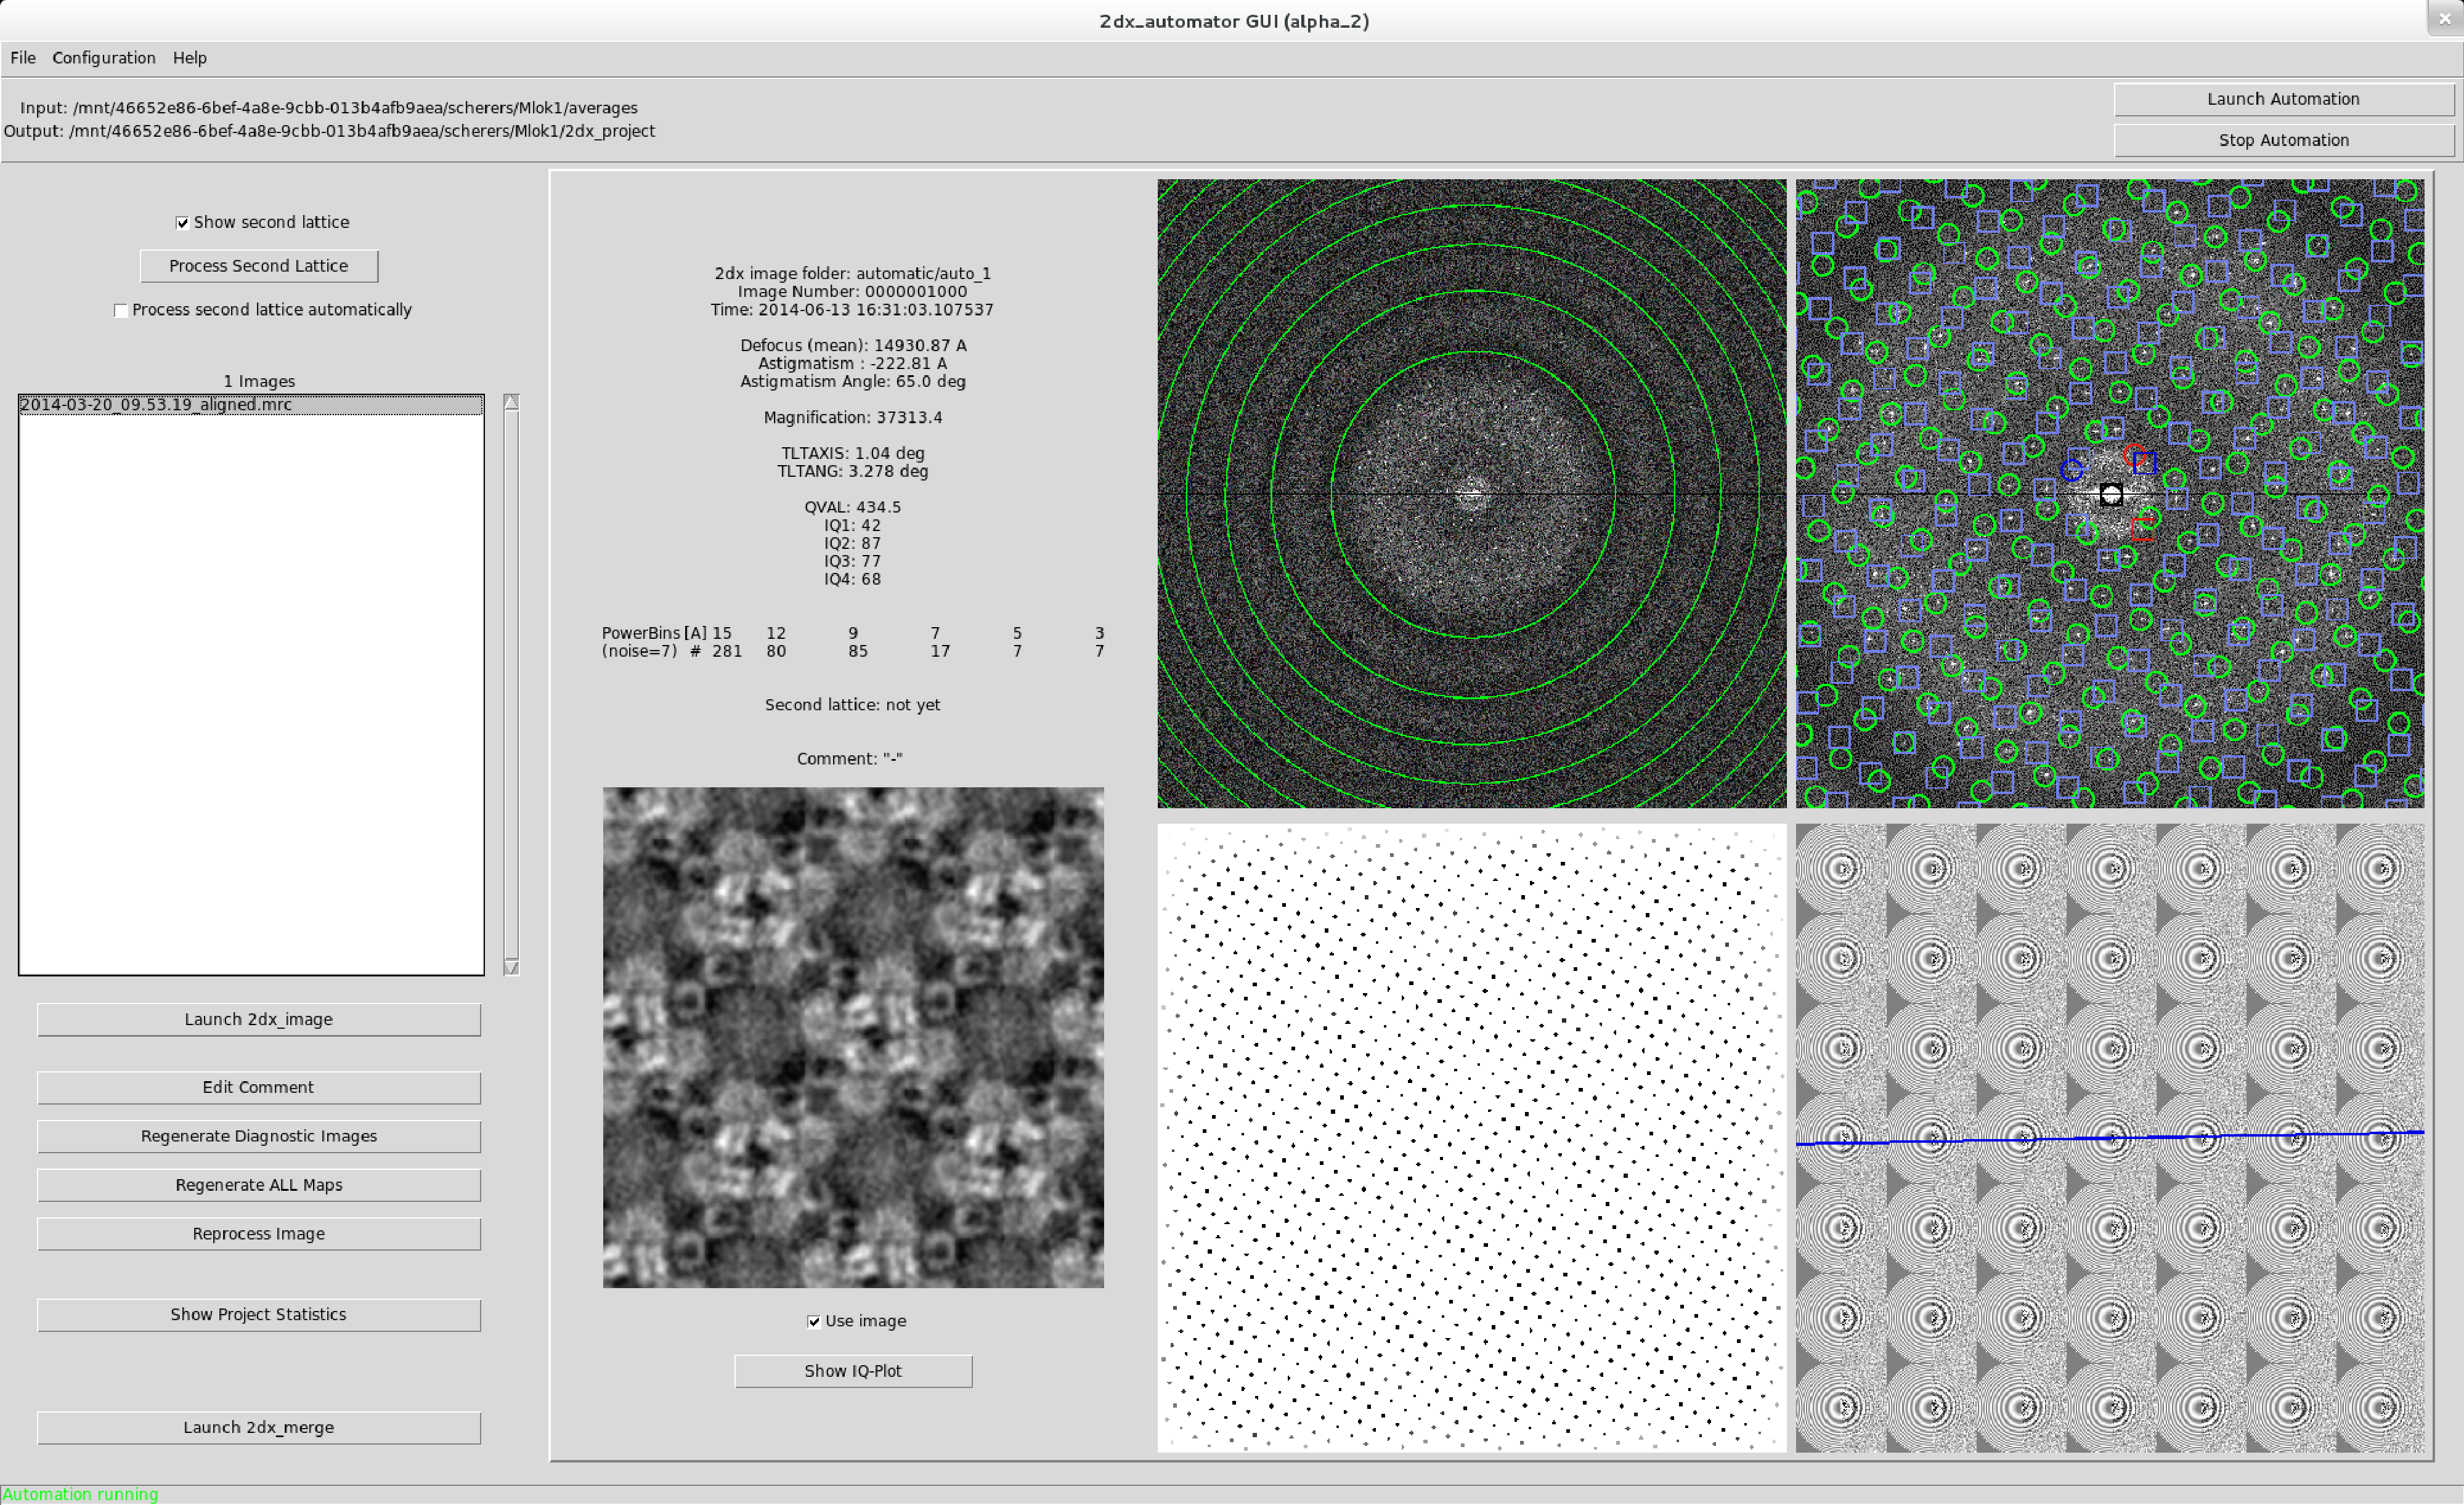
\includegraphics[width=1.0\textwidth]{auto.pdf}
	\caption{2dx\_automator}
	\label{fig:auto}
\end{figure}

\begin{figure}
	\centering
	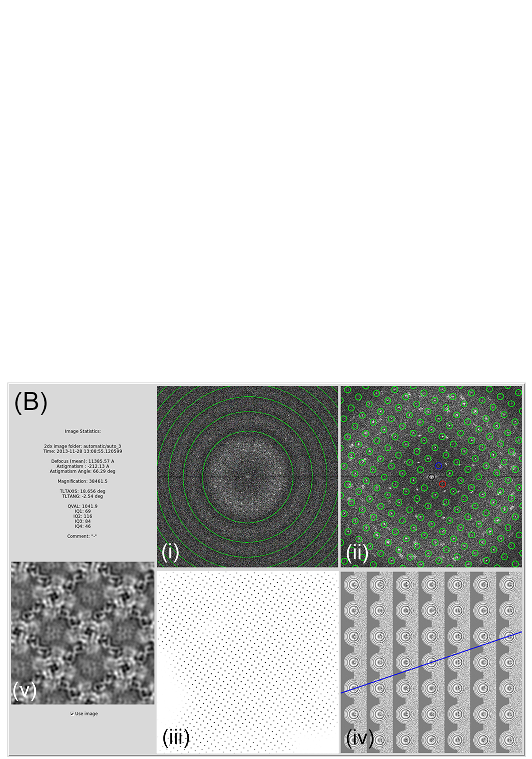
\includegraphics[width=1.0\textwidth]{auto2.pdf}
	\caption{2dx\_automator: Dia images}
	\label{fig:auto2}
\end{figure}


\subsection{Advanced tricks}

\begin{description}
	\item [Second lattice processing]
	\item [Manual processing intervention] 
	\item [Comment editing]
	\item [Updating image maps]
	\item [Reprocess an image]
	\item [Project statistics]
	\item [IQ-Stat analysis]
	\item [Configuration file handling] 
\end{description}



\begin{figure}
	\centering
	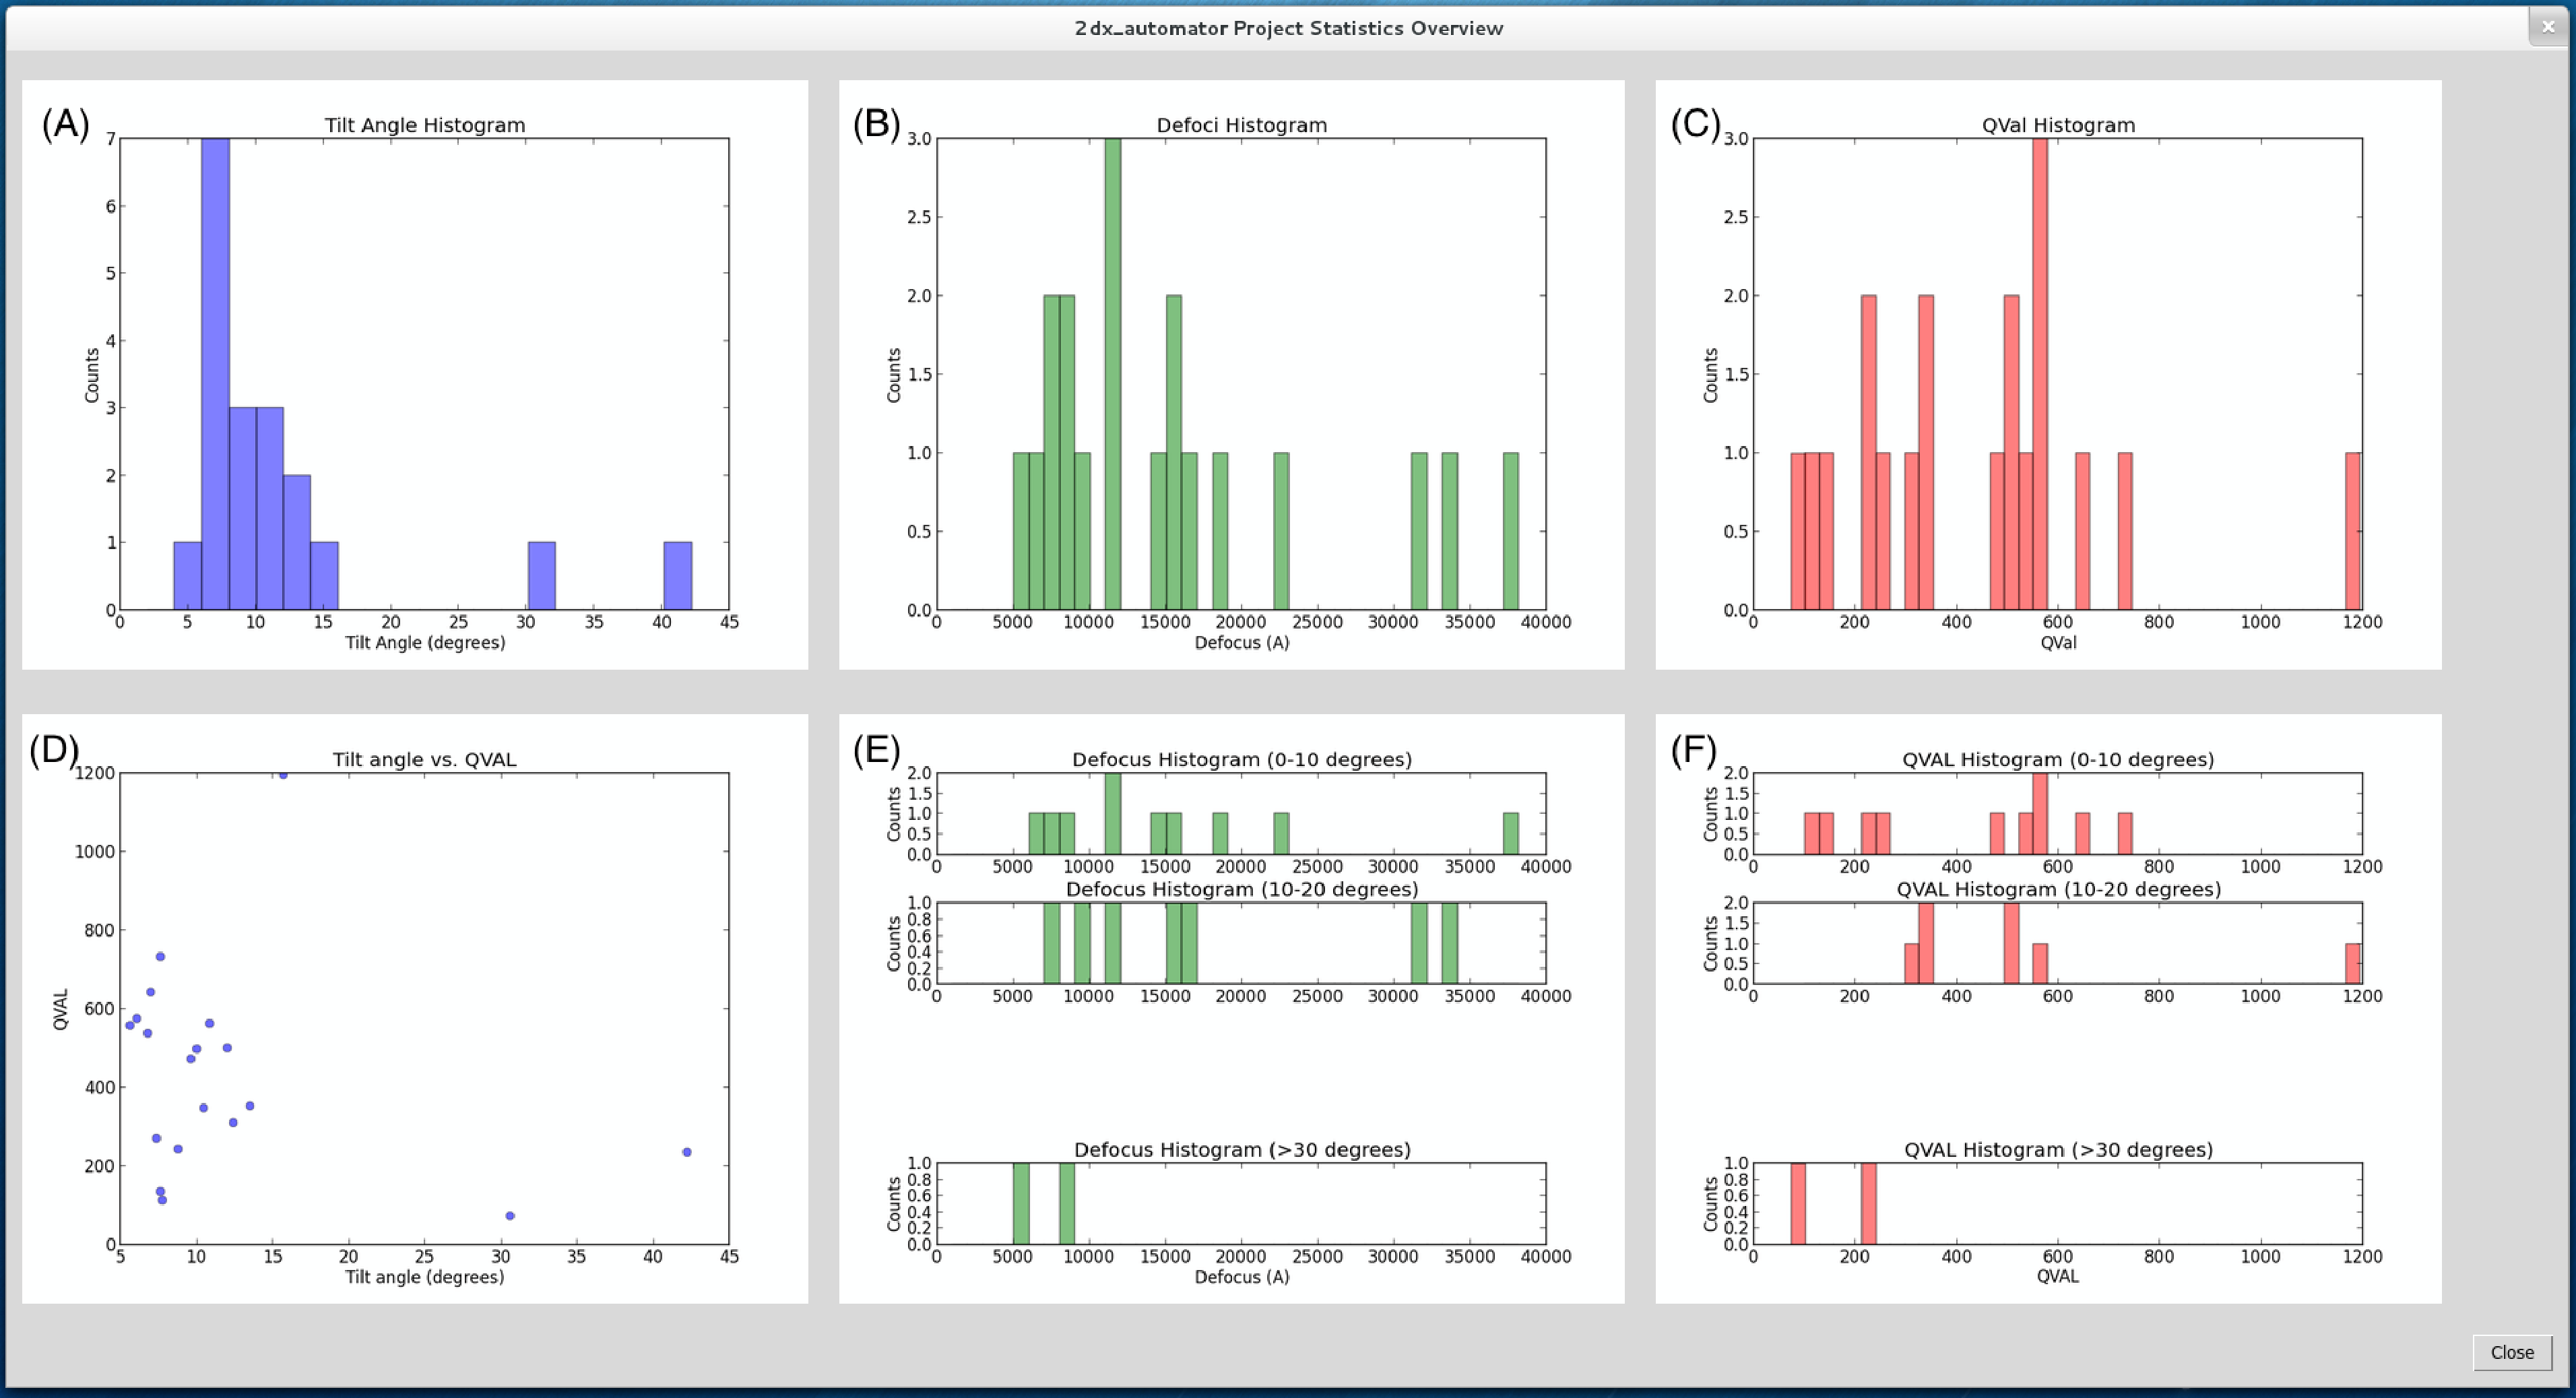
\includegraphics[width=1.0\textwidth]{auto_overview.pdf}
	\caption{Project stat}
	\label{fig:auto_stat}
\end{figure}